% Shared preamble for the CAWASMA viva notes (Atta, Asim, Neelam).
\documentclass[11pt,a4paper]{article}
\usepackage[T1]{fontenc}
\usepackage[utf8]{inputenc}
\usepackage{lmodern}
\usepackage{amsmath}
\usepackage{amssymb}
\usepackage{microtype}
\usepackage[margin=2.3cm]{geometry}
\usepackage{booktabs}
\usepackage{array}
\usepackage{tabularx}
\usepackage{longtable}
\usepackage{xcolor}
\usepackage{enumitem}
\usepackage{caption}
\usepackage{listings}
\usepackage{tikz}
\usetikzlibrary{arrows.meta,positioning,fit,backgrounds,calc}
\usepackage[hidelinks]{hyperref}

\definecolor{brand}{HTML}{1F4E79}
\definecolor{soft}{HTML}{F3F6F9}
\definecolor{rule}{HTML}{B8C2CC}
\definecolor{codebg}{HTML}{F7F8FA}
\definecolor{kw}{HTML}{1F5FA8}
\definecolor{cm}{HTML}{6A7684}

\captionsetup{font=small,labelfont={bf,color=brand},justification=raggedright,singlelinecheck=false}
\setlist{itemsep=2pt,topsep=3pt,parsep=0pt}
\sloppy
\hbadness=6000
\renewcommand{\arraystretch}{1.18}

% Code excerpts: small, wrapping, no language assumptions.
\lstset{
  basicstyle=\ttfamily\footnotesize,
  backgroundcolor=\color{codebg},
  frame=single, rulecolor=\color{rule},
  breaklines=true, breakatwhitespace=false,
  keywordstyle=\color{kw}\bfseries,
  commentstyle=\color{cm}\itshape,
  showstringspaces=false,
  columns=fullflexible,
  xleftmargin=6pt, xrightmargin=6pt,
  aboveskip=6pt, belowskip=6pt,
  literate={->}{{$\rightarrow$}}1 {<-}{{$\leftarrow$}}1,
}
\lstdefinestyle{py}{language=Python}

% Source footnote: where a fact came from in the repo.
\newcommand{\src}[1]{\footnote{Source: \texttt{#1}}}

% Person title block. \setperson{Name}{Role}{Roll}
\newcommand{\PersonName}{} \newcommand{\PersonRole}{} \newcommand{\PersonRoll}{}
\newcommand{\setperson}[3]{\renewcommand{\PersonName}{#1}\renewcommand{\PersonRole}{#2}\renewcommand{\PersonRoll}{#3}}

\newcommand{\maketitlepage}{%
\begin{titlepage}
\centering
\vspace*{1.2cm}
{\color{brand}\rule{\linewidth}{1.2pt}}\\[4mm]
{\Large\bfseries CAWASMA}\\[2mm]
{\large Context-Aware Web \& API Security Misconfiguration Analyzer}\\[3mm]
{\color{brand}\rule{\linewidth}{1.2pt}}\\[1.4cm]
{\large Final-year project --- viva study notes}\\[1.2cm]
{\Huge\bfseries \PersonName}\\[5mm]
{\large \PersonRole}\\[3mm]
{\large Roll number: \PersonRoll}\\[1.4cm]
\begin{tabular}{rl}
Supervisor: & Dr.\ Bilal Khan\\[2mm]
Team: & Asim Shakeel (22P-9229)\\
 & Neelam Jabeen (22P-9353)\\
 & Atta Ur Rehman (22P-9236)\\
\end{tabular}\\[1.2cm]
{\color{cm}\small These notes are generated from the repository, documentation and git history.\\
Every number is cited to the file or command it came from. Date: \today.}\\[1cm]
{\color{brand}\rule{\linewidth}{0.6pt}}
\end{titlepage}}

% A small helper for the "scoring in one line" boxes.
\newcommand{\keybox}[1]{\par\vspace{3pt}\noindent\fcolorbox{rule}{soft}{\parbox{\dimexpr\linewidth-2\fboxsep-2\fboxrule}{#1}}\par\vspace{3pt}}

\setperson{Atta Ur Rehman}{Backend \& scanner engine}{22P-9236}
\begin{document}
\maketitlepage
\tableofcontents
\clearpage

% Part A: the whole project. Shared, identical in all three documents.
\section{The whole project}

\subsection{The problem}
A normal security scanner gives a fixed severity to each kind of finding. A
missing \texttt{X-Content-Type-Options} header is ``medium'' wherever it is
found: on a public brochure page, and on a login API that returns credentials.
The person reading the report then has to work out, by hand, which of a hundred
``medium'' findings actually matters. That triage is slow and easy to get
wrong. Tools such as OWASP ZAP and Nuclei do find real issues, but they rate
the issue, not the place it sits in.\src{docs/supervisor/scanners.md}

\subsection{The idea}
CAWASMA scores the \emph{same} finding differently according to where it occurs
and what the endpoint returned. It does this with the standard CVSS v3.1
\emph{environmental} metrics, so the result is not an invented number: it is a
recomputation of the official score with a vector anyone can check on the FIRST
calculator.

\keybox{\textbf{One-paragraph pitch.} CAWASMA is a defensive, black-box,
HTTPS-only scanner for web apps and REST APIs. Each of its checks carries a
fixed CVSS v3.1 base vector. For every finding it works out how sensitive the
endpoint is (from the URL path) and what sensitive data the response holds
(credentials, personal data, financial data, internal IPs). It turns those into
CVSS environmental security requirements (CR/IR/AR) and recomputes the score, so
a login API and a public page that share a weakness no longer share a priority.
The point of the project is \emph{prioritisation, not detection}.}

\subsection{Architecture}
A scan is a pipeline. A URL goes in; a ranked, explained report comes out.

\begin{center}
\resizebox{0.98\linewidth}{!}{%
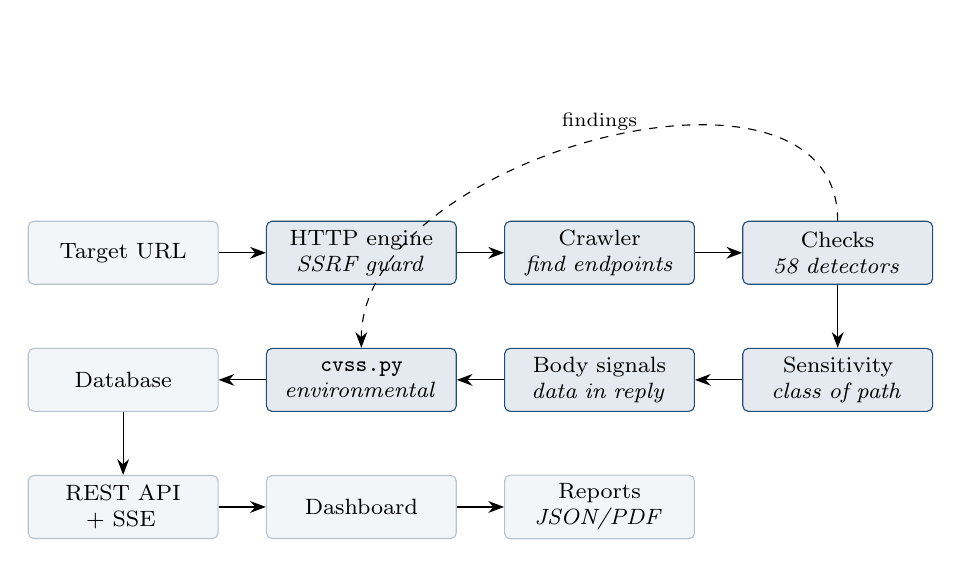
\begin{tikzpicture}[
  font=\footnotesize,
  >={Stealth[length=2mm]},
  box/.style={draw=rule,fill=soft,rounded corners=2pt,minimum height=8mm,inner sep=3pt,text width=22mm,align=center},
  core/.style={box,fill=brand!12,draw=brand},
  node distance=4mm and 6mm,
]
\node[box] (url) {Target URL};
\node[core,right=of url] (eng) {HTTP engine\\\textit{SSRF guard}};
\node[core,right=of eng] (crawl) {Crawler\\\textit{find endpoints}};
\node[core,right=of crawl] (checks) {Checks\\\textit{58 detectors}};
\node[core,below=8mm of checks] (sens) {Sensitivity\\\textit{class of path}};
\node[core,left=of sens] (body) {Body signals\\\textit{data in reply}};
\node[core,left=of body] (cvss) {\texttt{cvss.py}\\\textit{environmental}};
\node[box,left=of cvss] (db) {Database};
\node[box,below=8mm of db] (api) {REST API\\+ SSE};
\node[box,right=of api] (ui) {Dashboard};
\node[box,right=of ui] (rep) {Reports\\\textit{JSON/PDF}};
\draw[->] (url)--(eng); \draw[->] (eng)--(crawl); \draw[->] (crawl)--(checks);
\draw[->] (checks)--(sens); \draw[->] (sens)--(body); \draw[->] (body)--(cvss);
\draw[->] (cvss)--(db); \draw[->] (db)--(api); \draw[->] (api)--(ui); \draw[->] (ui)--(rep);
\draw[->,dashed] (checks.north) to[out=90,in=90] node[above,font=\scriptsize]{findings} (cvss.north);
\end{tikzpicture}}
\end{center}

\noindent The stages are: the \textbf{engine} fetches safely (one SSRF check per
redirect hop); the \textbf{crawler} discovers endpoints (seed, HTML, JavaScript,
a wordlist, and OpenAPI paths); the \textbf{checks} look for misconfigurations;
the \textbf{sensitivity} classifier labels each endpoint CRITICAL/HIGH/MEDIUM/LOW
from its path; the \textbf{body classifier} looks for sensitive data in the
reply; \texttt{cvss.py} turns those two into CR/IR/AR and recomputes the score;
the result is stored, served by the API over REST and Server-Sent Events, shown
on the dashboard, and exported as reports.

\subsection{Technology, and why}
\begin{center}
\small
\begin{tabularx}{\linewidth}{@{}p{34mm}X@{}}
\toprule
\textbf{Part} & \textbf{Choice and reason}\\
\midrule
Scanner core & Python 3.12 with \texttt{httpx} + \texttt{asyncio}: endpoints are analysed concurrently, and the core stays database-free so it is easy to test.\\
Scoring & The \texttt{cvss} library, so the environmental maths is the published CVSS v3.1 formula, not ours.\\
NLP & Sentence-Transformers (\texttt{all-MiniLM-L6-v2}) and spaCy for the sensitivity class; the engine still works with the built-in classifier when these are absent.\\
API & FastAPI, with Pydantic schemas and a frozen contract; Celery + Redis run scans in the background with live status.\\
Database & PostgreSQL in production, SQLite in tests; the models stay portable with a \texttt{JSONType} column and database-level cascades.\\
TLS & SSLyze (with a plain-\texttt{ssl} fallback) for the transport checks.\\
Reports & One HTML template through WeasyPrint for the PDF, so HTML and PDF never drift.\\
Frontend & Next.js 16 (App Router), React 19, TypeScript, Tailwind CSS v4, shadcn/ui, TanStack Query.\\
Tests & \texttt{pytest} (backend), Vitest + Testing Library and Playwright (frontend).\\
\bottomrule
\end{tabularx}
\end{center}

\subsection{Team roles and the shared contracts}
Three people own three areas, and they meet at three written contracts, frozen
so one person's change cannot silently break another's code.\src{CLAUDE.md; .github/CODEOWNERS}

\begin{center}
\small
\begin{tabularx}{\linewidth}{@{}p{24mm}X@{}}
\toprule
\textbf{Member} & \textbf{Owns}\\
\midrule
Asim (22P-9229) & Check specifications and their CVSS v3.1 vectors, the environmental mapping, chain templates, the sensitivity and response (ML/NLP) classifiers, and the whole evaluation lab.\\
Neelam (22P-9353) & The Next.js web app, the \texttt{frontend} service and its CI job.\\
Atta (22P-9236) & The backend: HTTP engine, crawler, check functions, CVSS scoring code, attack-chain engine, reports, FastAPI app, Celery workers, database and migrations, plus the shared infrastructure and reviews.\\
\bottomrule
\end{tabularx}
\end{center}

\begin{description}[leftmargin=0pt,itemsep=3pt]
\item[API contract (v1).] \texttt{app/api/schemas/contract.py} and
\texttt{docs/api-contract.md}: the field names the frontend reads
(\texttt{check\_id}, \texttt{base\_score}, \texttt{final\_score}, status
\texttt{DONE}).
\item[ML / CVSS contract.] \texttt{app/core/contracts.py} and
\texttt{docs/cvss-mapping-contract.md}: the types the engine and Asim's
classifiers exchange, so the engine keeps working with the built-in
classifiers when the ML packages are missing.
\item[Check-spec format.] \texttt{app/core/specs.py} and
\texttt{docs/check-spec-format.md}: how a check is declared so the registry can
run it.
\end{description}

\paragraph{Two scoring states.} Not every check is re-scored the new way yet.
Of 62 check ids, 25 have an approved specification and are scored through the
CVSS v3.1 environmental metrics; the other 37 still use an interim formula,
$\min(10,\ \text{base}\times\text{context multiplier}+\text{response bonus})$,
and each finding records which method scored it
(\texttt{scoring\_method}).\src{make coverage-stats; docs/06-scoring-model.md}

\clearpage

\section{What Atta built}
Atta owns the backend: everything that turns a URL into stored, scored, served
findings. The work is in \texttt{backend/app/core/} (the database-free scanner
logic), \texttt{backend/app/api/} (FastAPI), \texttt{backend/app/workers/}
(Celery), \texttt{backend/app/db/} and \texttt{backend/migrations/}, plus the
shared infrastructure (\texttt{docker-compose.yml}, \texttt{Makefile},
\texttt{.github/}).\src{.github/CODEOWNERS; CLAUDE.md}

\subsection{HTTP engine and the SSRF guard}
\textbf{What it does.} The engine (\texttt{core/engine.py}) makes every network
request for a scan. It keeps the scan inside one host, follows redirects safely,
and refuses to touch private or internal addresses. The safety logic lives in
\texttt{utils/security.py}.

\textbf{How it works.}
\begin{itemize}
\item \texttt{HttpEngine(scope\_host=\dots)} fetches with \texttt{httpx} and
\texttt{asyncio}. Plain GET/HEAD are cached per scan by \texttt{fetch()}, so the
same URL is not fetched twice.
\item Before each connection, \texttt{resolve\_and\_validate()} resolves the host
and checks \emph{every} resolved IP with \texttt{\_ip\_is\_disallowed()}. A
redirect is a new hop, so the check runs again for the next host.
\item \texttt{PinnedNetworkBackend} connects to the exact IP that was validated,
so DNS cannot change between the check and the connection (DNS rebinding).
\item The engine keeps no cookies between requests and records \texttt{Set-Cookie}
metadata (never values) on every hop. In passive mode it sends only GET/HEAD.
\end{itemize}

\begin{lstlisting}[style=py,caption={SSRF block list on the resolved IP (\texttt{utils/security.py}).}]
def _ip_is_disallowed(ip, *, internal_ok=False):
    inner = _embedded_ipv4(ip)        # unwrap ::ffff:a.b.c.d
    if inner is not None:
        r = _ip_is_disallowed(inner, internal_ok=internal_ok)
        return f"{r} (via {ip})" if r else None
    if ip in METADATA_IPS: return "cloud metadata address"
    if ip.is_loopback:     return "loopback address"
    if ip.is_link_local:   return "link-local address"
    if ip.is_reserved:     return "reserved address"
    if internal_ok:        return None   # tests / eval only
    if ip.is_private:      return "private address"
    return None
\end{lstlisting}

\begin{center}
\resizebox{0.98\linewidth}{!}{%
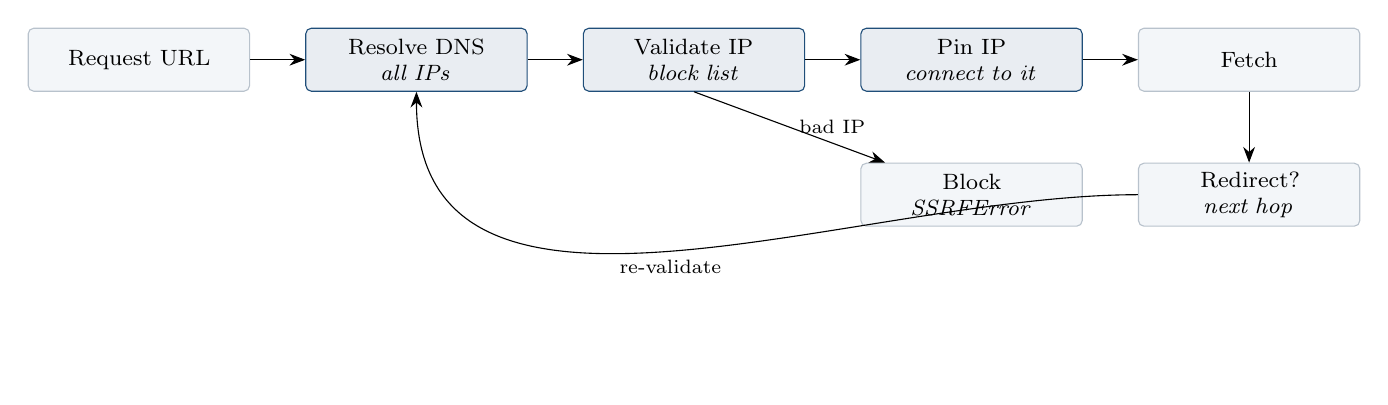
\begin{tikzpicture}[font=\footnotesize,>={Stealth[length=2mm]},
  s/.style={draw=rule,fill=soft,rounded corners=2pt,text width=26mm,align=center,minimum height=8mm,inner sep=3pt},
  d/.style={draw=brand,fill=brand!10},
  node distance=4mm and 7mm]
\node[s] (req){Request URL};
\node[s,d,right=of req] (res){Resolve DNS\\\textit{all IPs}};
\node[s,d,right=of res] (val){Validate IP\\\textit{block list}};
\node[s,d,right=of val] (pin){Pin IP\\\textit{connect to it}};
\node[s,right=of pin] (ok){Fetch};
\node[s,below=9mm of pin] (block){Block\\\textit{SSRFError}};
\node[s,below=9mm of ok] (hop){Redirect?\\\textit{next hop}};
\draw[->](req)--(res);\draw[->](res)--(val);\draw[->](val)--(pin);\draw[->](pin)--(ok);
\draw[->](val.south)--(block) node[midway,right,font=\scriptsize]{bad IP};
\draw[->](ok)--(hop);
\draw[->](hop) to[out=180,in=270] node[below,font=\scriptsize]{re-validate} (res.south);
\end{tikzpicture}}
\end{center}

\textbf{Design decisions.} Validating the \emph{resolved IP} (not the hostname)
and pinning it is what stops DNS rebinding; a hostname check alone would not.
\texttt{allow\_private} exists only for tests and the evaluation harness, where
the targets are on a private Docker network; in normal runs
\texttt{ALLOWED\_INTERNAL\_HOSTS} is empty.

\textbf{Inputs/outputs.} In: a URL and the scan scope. Out: a validated
\texttt{ScanResponse} used by the crawler and the checks. \textbf{Tested by}
\texttt{tests/security/} (loopback, link-local, metadata, IPv4-mapped IPv6, and
rebinding cases) and \texttt{tests/unit} engine tests.

\textbf{Limitations.} The guard blocks by IP class; a public host that an
attacker controls and that itself proxies inward is out of scope, as is any
target that requires a login.

\subsection{Crawler}
\textbf{What it does.} \texttt{core/crawler.py} discovers endpoints to scan from
a single seed URL.

\textbf{How it works.} It reads the seed page, follows in-scope HTML links,
extracts routes from JavaScript, tries a wordlist, and reads OpenAPI/Swagger GET
paths and \texttt{/rest/}, \texttt{/vN/} routes. \texttt{\_state\_changing()}
blocks anything named like an action (\texttt{/createdb}, \texttt{/logout},
\texttt{/reset}) so the scan never changes server state. A soft-404 baseline
stops pages that answer 200-but-empty from being treated as real endpoints.

\textbf{Design decisions.} Discovery is deterministic (fixed order) so a scan is
reproducible. Only GET/HEAD are used to discover. \textbf{Tested by} crawler
unit tests and \texttt{tests/unit/test\_scan\_performance.py} (state-changing
route recognition). \textbf{Limitation:} no JavaScript execution, so routes that
only appear after client-side rendering are missed.

\subsection{Check framework and detection functions}
\textbf{What it does.} A check is a pure function
\texttt{detect(ctx: CheckContext) -> RawFinding | None}, registered with
\texttt{@rule}. Atta writes the detection functions (one module per category in
\texttt{core/checks/}); Asim owns the catalog entry and CVSS vector.

\textbf{How it works.} The registry (\texttt{core/checks/registry.py}) also runs
the newer \emph{spec-driven} checks from \texttt{config/checks.yaml} with a
\texttt{SpecContext}. A guard test fails if a check has no fire/no-fire test.
There are 58 catalog checks; \texttt{checks.yaml} adds 4 spec-only ids, 62 in
all.\src{make check-coverage; backend/app/core/checks/}

\textbf{Design decision.} Keeping \texttt{core/} database-free means a check reads
only its \texttt{CheckContext} and can be unit-tested with no server.
\textbf{Tested by} \texttt{tests/checks/} (a fire and a no-fire test per check).

\subsection{CVSS scoring code}
\textbf{What it does.} \texttt{core/cvss.py} is the scoring engine. It computes
the environmental (context-aware) score from a base vector plus the endpoint
class and body signals, and it keeps the interim legacy formula for checks that
do not yet have a spec.

\textbf{How it works.} \texttt{environmental\_score()} builds the full CVSS
vector by appending CR/IR/AR, then uses the \texttt{cvss} library to compute both
base and environmental scores, so the maths is the published formula. The
requirements themselves come from Asim's mapping via
\texttt{security\_requirements()}. \texttt{score\_finding()} looks up the check's
base vector from the spec registry.

\begin{lstlisting}[style=py,caption={Append CR/IR/AR, recompute with the \texttt{cvss} library (\texttt{core/cvss.py}).}]
reqs, reasons = security_requirements(sensitivity, signals, mapping)
tail = "".join(f"/{m}:{reqs[m]}" for m in ("CR", "IR", "AR"))
scored = CVSS3(base_vector + tail)
base, final = scored.base_score, scored.environmental_score
if all(v == "X" for v in reqs.values()):
    reasons.append("no-context-change")   # public: base stands
\end{lstlisting}

\keybox{\textbf{Why not our own formula?} Because then the number would be ours
to defend. By appending CR/IR/AR to the official base vector and letting the
\texttt{cvss} library compute it, the final score is a standard CVSS v3.1
environmental score that anyone can reproduce on the FIRST calculator. Our only
claim is the \emph{mapping} from context to CR/IR/AR.}

\textbf{Inputs/outputs.} In: a check's base vector, the sensitivity class, the
body signals, and Asim's mapping. Out: a \texttt{ContextScore} (base, final,
severity bucket, the full vector, and the \texttt{score\_reasons}) stored on the
finding. \textbf{Tested by} \texttt{tests/unit/test\_cvss.py}.
\textbf{Limitation:} the 37 legacy checks are not on this path yet; they record
\texttt{scoring\_method = legacy}.

\subsection{Attack-chain engine}
\textbf{What it does.} \texttt{core/chains.py} correlates several findings into
one attack chain and scores it with a composite vector.

\textbf{How it works.} \texttt{correlate()} reads the templates from
\texttt{config/chains.yaml} (Asim's file), groups findings by scope unit, and
emits a \texttt{DetectedChain} per matched template. Each member's evidence names
the chain. \textbf{Tested by} \texttt{tests/unit/test\_chains.py}.
\textbf{Limitation:} chains only form where a template matches; on the four
evaluation targets they appear only on DVWA and crAPI.

\subsection{Pipeline orchestration}
\textbf{What it does.} \texttt{core/pipeline.py} is the conductor:
\texttt{run\_pipeline()} drives crawl $\rightarrow$ checks $\rightarrow$ classify
$\rightarrow$ score $\rightarrow$ chains and produces a \texttt{ScanResult}.

\textbf{How it works.} It analyses endpoints concurrently with a bounded limit
(\texttt{MAX\_CONCURRENT\_ENDPOINTS}) in a fixed order, so a scan is both fast and
reproducible. \texttt{\_analyse\_endpoint()} runs the checks for one endpoint,
asks for its sensitivity class and body signals, and scores each finding.
\texttt{StageClock} records per-stage timings into \texttt{stats[stage\_seconds]}.
Progress is written to \texttt{Scan.progress\_detail} after each step, and
\texttt{cancel\_requested} is checked there too. An unreachable target raises
\texttt{ScanError} --- the only error text shown to users.

\textbf{Design decision.} The pipeline is the one place that depends on both the
engine and the classifiers, so it holds the fallback logic
(\texttt{\_ml\_classifier()}): if the ML classifier is absent it uses the
built-in one, honouring the contract. \textbf{Tested by}
\texttt{tests/integration/} (full scans against fixtures).
\textbf{Limitation:} a very large site is bounded by \texttt{SCAN\_TIMEOUT}
rather than scanned exhaustively.

\subsection{FastAPI application and the API}
\textbf{What it does.} \texttt{api/} exposes the scanner over REST and
Server-Sent Events. \texttt{POST /api/scan} starts a scan; other routes read
results, a single finding, history, and exports.

\textbf{How it works.}
\begin{itemize}
\item \texttt{services/scan\_dispatch.py} queues the scan on Celery with the task
id equal to the scan id, returning 503 \texttt{QUEUE\_UNAVAILABLE} if the broker
is down. \texttt{RUN\_SCANS\_INLINE} runs it as a FastAPI background task instead.
\item Live status is SSE at \texttt{GET /api/scan/\{id\}/events}, which reads the
database (at most \texttt{SSE\_MAX\_STREAMS\_PER\_CLIENT} open per client).
\item Cancel sets \texttt{Scan.cancel\_requested}. Scanning is rate-limited with a
Redis fixed window (429; \texttt{api/limits.py}).
\item Errors use the envelope
\texttt{\{success:false, error:\{code,message\}\}}. Routes return Pydantic
schemas from \texttt{api/schemas/}, never ORM objects.
\end{itemize}

\textbf{Design decision.} The contract field names
(\texttt{check\_id}, \texttt{base\_score}, \texttt{final\_score}) are mapped in
\texttt{api/schemas/} rather than renaming database columns, so the database and
the API can evolve separately. \textbf{Tested by} \texttt{tests/api/} (contract
schemas, the OpenAPI export, and the documented examples).
\textbf{Limitation:} SSE needs a database read loop; there is no push from the
worker, so status lags by at most one poll interval.

\subsection{Celery workers}
\textbf{What it does.} \texttt{workers/} runs scans off the request thread.
\texttt{cawasma.run\_scan} executes the pipeline and writes results.

\textbf{How it works.} At start-up the API marks any \texttt{api}-runner scan
still QUEUED/RUNNING as FAILED (it died with the old process); Celery scans carry
\texttt{options.runner = "celery"}. The task id is the scan id, so status and
cancel line up. \textbf{Tested by} worker and dispatch tests.
\textbf{Limitation:} a worker crash mid-scan leaves a scan to be reaped at the
next start-up rather than resumed.

\subsection{Database and migrations}
\textbf{What it does.} \texttt{db/} holds the SQLAlchemy models and session;
\texttt{migrations/} holds the Alembic history (0001--0005).

\textbf{How it works.} Models stay portable so the same code runs on SQLite (in
tests) and PostgreSQL (in production): JSON columns use \texttt{JSONType} (JSONB
on PostgreSQL), and deletes rely on database \texttt{ON DELETE} cascades, which
are enforced on SQLite too. The official base score and the context-aware score
are separate columns on the \texttt{findings} table.

\textbf{Design decision.} Schema changes go through \texttt{alembic
revision --autogenerate}; a merged migration is never edited and tables are never
created by hand, so every environment has the same schema. \textbf{Tested by}
\texttt{tests/db/} and the CI Alembic upgrade/downgrade. \textbf{Limitation:}
keeping two databases portable rules out some PostgreSQL-only features.

\subsection{Reports}
\textbf{What it does.} \texttt{core/reports.py} renders a scan as JSON, CSV, HTML
or PDF, with no database access (it takes an assembled data dictionary from
\texttt{services/report\_service.py}).

\textbf{How it works.} \texttt{score\_story()} turns a finding's
\texttt{score\_reasons} into the plain-English ``why this score'' lines; HTML and
PDF both come from \texttt{app/templates/report.html.j2}, the PDF being that same
HTML through WeasyPrint, so the two can never drift. \texttt{redact\_evidence()}
runs again on every export.

\textbf{Design decision.} Keeping the renderers database-free means a report can
be produced and unit-tested from a fixture. \textbf{Tested by} report unit tests.
\textbf{Limitation:} the PDF depends on WeasyPrint's CSS support, so the template
avoids layout features it renders poorly.

\section{Numbers to know}
All figures are from the repository at commit \texttt{7cc819f} on \texttt{main}.

\subsection{Detection vs.\ ZAP and Nuclei}
Four deliberately vulnerable targets, each tool scored only on the checks its
rules map to.\src{eval/results/metrics.csv; eval/results/final/tools.md}
\begin{center}\small
\begin{tabular}{@{}llrrrrrr@{}}
\toprule
Tool & scope & TP & FP & FN & Precision & Recall & Time (s)\\
\midrule
CAWASMA & all (micro) & 25 & 0 & 8 & 1.00 & 0.758 & 10.5\\
ZAP (baseline) & all (micro) & 7 & 0 & 14 & 1.00 & 0.333 & 104.4\\
Nuclei & all (micro) & 13 & 0 & 4 & 1.00 & 0.765 & 126.2\\
\bottomrule
\end{tabular}
\end{center}
Per-target CAWASMA recall: Juice Shop 0.44, DVWA 1.00, VAmPI 0.75, crAPI 0.83.
Read these carefully: ZAP ran passively (no attacks), and the ground truth uses
CAWASMA's check ids, which favours CAWASMA's scope.

\subsection{Coverage, scoring split and tests}
\begin{center}\small
\begin{tabular}{@{}lr@{}}
\toprule
Metric & Value\\
\midrule
Check ids (catalog 58 + 4 spec-only) & 62\\
With an approved spec / scored environmental & 25\\
Scored by the legacy interim formula & 37\\
Latest eval findings (4 targets) & 1230\\
\quad environmental / legacy & 765 (62\%) / 465 (38\%)\\
Backend tests (pytest) & 978\\
Frontend unit test files / e2e specs & 25 / 7\\
\bottomrule
\end{tabular}
\end{center}
\hfill\textit{\footnotesize Source: \texttt{make coverage-stats}; pytest collection; \texttt{git ls-files}.}

\subsection{Ranking result, honestly}
NDCG@10 on environmentally-scored findings, base vs.\ context, mean over 1000
tie-breaks (seed 13).\src{eval/results/final/ranking\_environmental.md}
\begin{center}\small
\begin{tabular}{@{}lrr@{}}
\toprule
Target & base & context\\
\midrule
Juice Shop & 0.001 & 0.000\\
DVWA & 0.147 & 0.261\\
VAmPI & 0.607 & 0.591\\
crAPI & 0.539 & 0.535\\
\textbf{Mean} & \textbf{0.324} & \textbf{0.347}\\
\bottomrule
\end{tabular}
\end{center}
\textbf{What this means.} On four targets the context-aware ranking beats the
base score only on DVWA and is otherwise equal or slightly worse. So the
evaluation does \emph{not} show the ranking is better overall. The graded pools
are not finished, so there is no pool-based NDCG yet. The honest claim the
project proves is the \emph{mechanism}: the same weakness on a sensitive,
credential-returning endpoint is scored higher than on a public page, with a
reproducible CVSS vector.

\section{Contribution timeline}
Grouped from merged pull requests.\src{gh pr list (upstream); git log}
\begin{center}\small
\begin{tabularx}{\linewidth}{@{}llX@{}}
\toprule
Merged & PRs & What changed\\
\midrule
May--24 Oct & \#1--\#5, \#7 & Project scaffold, database layer, API contracts.\\
25 Oct & \#13--\#16 & ML stubs where the contract expects them; data-model and contract gaps.\\
25 Oct & \#22, \#23 & Async engine and crawler; hardened SSRF guard, \texttt{ALLOWED\_INTERNAL\_HOSTS}.\\
25--26 Oct & \#24, \#25 & Check registry; CVSS v3.1 environmental scoring from sensitivity + body signals.\\
26 Oct & \#26, \#27 & Vertical slice; stop tracking the local database.\\
26--27 Oct & \#36, \#39 & Whole-code bug sweep; full check set.\\
4 Nov & \#45 & Celery scans, live SSE status, cancel, rate limit.\\
4--5 Nov & \#52, \#53, \#57 & Final audit (no code changed in phase 1).\\
5 Nov & \#65, \#67 & Fix \texttt{validate-config} crash and the PostgreSQL CI job.\\
5--9 Nov & \#68, \#74, \#76--\#79 & CODEOWNERS; \texttt{make up} runs the whole app; supervisor docs; docs cleanup.\\
\bottomrule
\end{tabularx}
\end{center}
\textbf{Reviews given.} Atta also pushed fixes inside teammates' folders on
\texttt{atta/fix-*} branches for the owner to review: for Asim \#56, \#58, \#60,
\#61, \#62, \#70, \#71, \#72; for Neelam \#54, \#59, \#63, \#64, \#66, \#73, \#75.

\section{Viva preparation}
\subsection{Likely questions, with short answers}
\begin{enumerate}[leftmargin=*,itemsep=3pt]
\item \textbf{How do you stop SSRF?} Resolve the host, check every resolved IP
against a block list (loopback, link-local, private, reserved, cloud metadata,
IPv4-mapped IPv6), then connect to that pinned IP so DNS cannot change. The check
re-runs on every redirect hop.
\item \textbf{What is DNS rebinding and how do you handle it?} The host resolves
to a safe IP at check time and a dangerous one at connect time.
\texttt{PinnedNetworkBackend} connects to the IP we validated, so the two cannot
differ.
\item \textbf{Why async httpx?} Endpoints are analysed concurrently with a
bounded limit, so scans stay fast (mean 10.5\,s per target) without threads.
\item \textbf{Why is \texttt{core/} database-free?} So a check is a pure function
of its \texttt{CheckContext} and can be unit-tested with no database or network.
\item \textbf{Why not invent your own score?} The final number is a standard CVSS
v3.1 environmental score computed by the \texttt{cvss} library; only the mapping
to CR/IR/AR is ours, and it is auditable.
\item \textbf{Base vs.\ final score --- why keep both?} The official base score
must stay visible; the context-aware score sits next to it, never replacing it.
\item \textbf{The ranking isn't better --- so what does the project prove?} It
proves the mechanism works and is reproducible: a weakness on a sensitive,
credential-bearing endpoint scores higher than on a public page. The ranking
study is honest that, on four targets, it is not better overall.
\item \textbf{How does a scan run in the background?} \texttt{POST /api/scan}
queues a Celery task (task id = scan id); progress is written to the database and
streamed by SSE; cancel sets a flag checked at each step.
\item \textbf{What happens if the broker is down?} The queue endpoint returns 503
\texttt{QUEUE\_UNAVAILABLE}; \texttt{RUN\_SCANS\_INLINE} can run the scan in the
API process instead.
\item \textbf{How do you avoid changing the target?} Only GET/HEAD/OPTIONS, and
the crawler never requests routes named like actions (\texttt{/logout},
\texttt{/createdb}).
\item \textbf{How is the PDF report produced?} One HTML template through
WeasyPrint, so HTML and PDF cannot drift; every export redacts evidence again.
\item \textbf{How do you keep secrets out of logs and reports?}
\texttt{utils/redaction.py} redacts before anything is logged, stored or
reported; cookies store metadata, never values.
\item \textbf{Why both SQLite and PostgreSQL?} SQLite for fast tests, PostgreSQL
in production; models stay portable with \texttt{JSONType} and database-level
cascades.
\item \textbf{How do migrations work?} Alembic autogenerate; a merged migration
is never edited; tables are never created by hand.
\item \textbf{What is soft-404 handling?} The crawler learns a baseline for
``not found'' pages that still return 200, so they are not scanned as real
endpoints.
\item \textbf{Why is XSS/BOLA not covered?} Confirming them needs attack payloads
or logged-in accounts, which breaks the safe, read-only, unauthenticated design.
BOLA depends on authenticated scanning, which is future work.
\item \textbf{How would you scale this?} Scans are already Celery tasks; add
workers horizontally. The engine bounds concurrency per scan; the database and
Redis are the shared state.
\item \textbf{How is a scan cancelled mid-run?} \texttt{Scan.cancel\_requested}
is set and checked at every progress step, so the pipeline stops cleanly.
\item \textbf{What is the scope guarantee?} \texttt{HttpEngine(scope\_host=...)}
makes no request to another host and follows no redirect off it.
\item \textbf{How are endpoints scored concurrently but deterministically?}
Concurrency is bounded and the order is fixed, so results are reproducible.
\item \textbf{What does \texttt{scoring\_method} record?} Whether a finding was
scored by the CVSS environmental metrics or by the legacy interim formula.
\item \textbf{How do you test the checks?} Every check has a fire and a no-fire
test in \texttt{tests/checks/}; a guard test fails if one is missing.
\item \textbf{What stops a check from being too slow?} Plain GET/HEAD are cached
per scan, and per-stage timings are recorded in \texttt{stats[stage\_seconds]}.
\item \textbf{How do you handle an unreachable target?} The pipeline raises
\texttt{ScanError}, the scan is marked FAILED, and only that message is shown.
\item \textbf{Where does the sensitivity class come from in the pipeline?} From
\texttt{app.ml.sensitivity.classify} (Asim) through the contract, with the
built-in classifier as a fallback.
\item \textbf{What is the single biggest risk in your code?} The SSRF guard: a
gap there would let a scan reach internal services, so it has the most tests.
\end{enumerate}

\subsection{Three-minute demo script}
\begin{enumerate}[leftmargin=*]
\item Start the stack (\texttt{make up}) and open the app. Say: ``A scan is a
Celery task; the API streams live status over SSE.''
\item Scan a target. Point at the live progress and the stage timings.
\item Open a finding's detail. Show the base score, the final score, and the CVSS
vector with CR/IR/AR appended. Say: ``The number is a standard CVSS v3.1
environmental score, not ours.''
\item Export the PDF. Say: ``Same HTML through WeasyPrint; evidence is redacted
again on export.''
\item Show the SSRF test file briefly. Say: ``Every resolved IP is validated and
pinned on every hop.''
\end{enumerate}

\subsection{Five things to explain without notes}
\begin{enumerate}[leftmargin=*]
\item The SSRF guard: resolve, validate every IP, pin it, re-check each hop.
\item \texttt{environmental\_score()}: append CR/IR/AR, recompute with the
\texttt{cvss} library.
\item Why the base score is always kept next to the final score.
\item The scan lifecycle: queue $\rightarrow$ Celery $\rightarrow$ SSE status
$\rightarrow$ cancel flag $\rightarrow$ stored findings.
\item The honest ranking result and what the project really proves.
\end{enumerate}

% Part F: glossary. Shared, identical in all three documents.
\section{Glossary}
\begin{description}[leftmargin=0pt,style=nextline,itemsep=3pt]
\item[CVSS base score] The standard severity of a vulnerability on its own, 0--10,
from a vector such as \texttt{AV:N/AC:L/\dots}. Fixed per check; never invented per scan.
\item[CVSS environmental score] The base score recomputed for a particular
environment, using CR/IR/AR and modified base metrics. CAWASMA's context-aware
score is this.
\item[CR / IR / AR] Confidentiality, Integrity and Availability \emph{Requirements}:
environmental inputs saying how much each property matters here. Values Low,
Medium, High, or X (Not Defined). CAWASMA sets them from the endpoint class and
the data in the response.
\item[Sensitivity class] CAWASMA's label for how sensitive an endpoint is ---
CRITICAL, HIGH, MEDIUM or LOW --- from the words in its URL path.
\item[Body signals] Sensitive data found in a response: credentials, personal
data (PII), financial data, or an internal IP address. Evidence is redacted.
\item[Base vs.\ final score] CAWASMA always keeps both: the official base score
and the context-aware (environmental) final score, in separate columns.
\item[Legacy vs.\ environmental scoring] A finding is scored either by the CVSS
environmental metrics (approved specs) or by the interim legacy formula; its
\texttt{scoring\_method} says which.
\item[Precision] Of the findings that were judged, the fraction that were
correct: $\text{TP}/(\text{TP}+\text{FP})$.
\item[Recall] Of the real issues in the answer key, the fraction found:
$\text{TP}/(\text{TP}+\text{FN})$.
\item[FPR] False-positive rate: $\text{FP}/(\text{FP}+\text{TN})$.
\item[Ground truth] A hand-written list, per target, of which check should
(\texttt{present}) or should not (\texttt{absent}) fire on which endpoint.
\item[NDCG@10] Normalised Discounted Cumulative Gain at rank 10: a score for how
well a ranking puts the important items near the top, against a graded list.
\item[Tie-break sampling] Base scores tie often, so a ranking's NDCG is averaged
over 1000 random orderings of the tied items, with a fixed seed.
\item[SSRF] Server-Side Request Forgery: tricking the scanner into requesting an
internal address. CAWASMA guards against it by validating the resolved IP on
every hop.
\item[Soft-404] A page that returns HTTP 200 but is really ``not found''. The
crawler learns a baseline so it does not treat these as real endpoints.
\item[Passive vs.\ active scan] Passive sends only safe GET/HEAD and reads what
comes back; active sends extra, still non-destructive, probes. CAWASMA never
sends attack payloads.
\item[BOLA / IDOR] Broken Object-Level Authorisation / Insecure Direct Object
Reference: reading another user's object by changing an id. CAWASMA only flags an
\emph{indicator}; confirming it needs logged-in accounts, which is future work.
\item[Attack chain] Several findings that together make a bigger risk, correlated
from a template and scored with their own composite vector.
\item[Environmental metric ``X''] ``Not Defined'': the neutral baseline. A public
(LOW) endpoint uses X, so its score is unchanged --- context only ever raises a
score here, it does not lower a public page below its base.
\end{description}

\end{document}
